\chapter{Optimal Smooth Paths Based on Clothoids for Car-like Vehicles in the Presence of Obstacles}
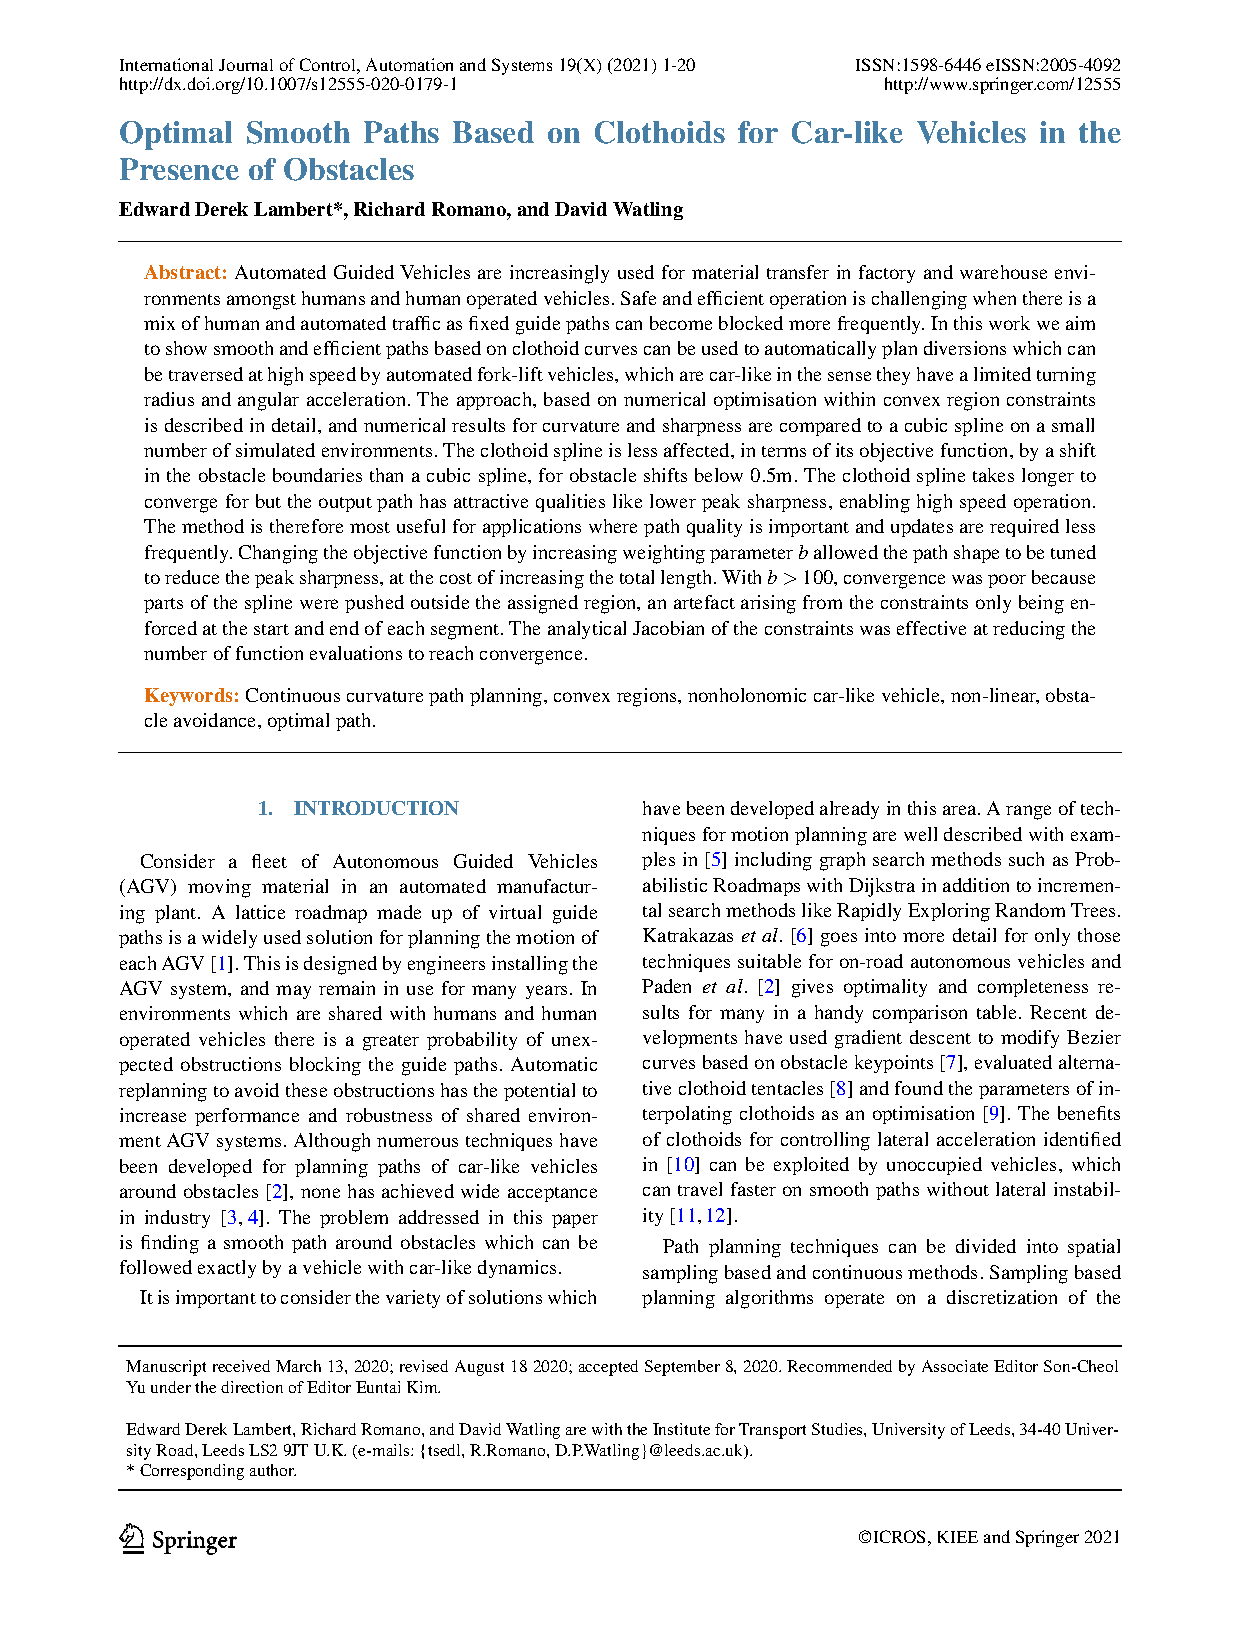
\includepdf[pages=-]{2021_192_20-00179-12March2021.pdf}

\section{Bits of \LaTeX advice}

\begin{enumerate}
	\item Do look at the output log and try to understand any errors - they are sometimes important!
	\item In the final pdf, do a search for ? - it is what \LaTeX will give when a reference is missing. Having missing references in your submitted thesis is, at best, embarrassing and potentially a failing matter.
	\item A good quality bib file is important - make sure that entries are consistent in whether journals are abbreviated, capitalised and how Author names are presented. A good way to do this is to use Mendeley to import your bib file and then use its doi lookup feature which will re-write your bibliography entries in a standardised form. You then export the bibliography back oit as a bib file.
	\item Be particularly careful about older papers where the doi may not be easy to track down. Also watch out for JETP Letters that you are being consistent in citing the English language version (or the Russian, but don't mix and match!)
	\item Although \LaTeX guides may show you how to assemble a multi-part figure from within \LaTeX, it can be hard to make sub-plots appear exactly the same size. We recommend using something like Inkscape to assemble the parts of a figure and lay them out nicely. Be careful if saving to pdf files thatr the fonts are preserved - otherwise you can lose greek symbols.
	\item If preparing figures in Origin, set the plot size to be exactly the right size or exactly double size and then scale fonts and symbols accordingly. Use Origin's ability to copy formatting between graphs to make everything nicely consistent (e.g. frame sizes, thicknesses, colour schemes, point sizes and shapes).
	\item In general resist the temptation to put [H] when placing figures and tables - in most cases it is better to let \LaTeX work out where to put things. It can get tricky if you have a lot of figures one after another (perhaps a single multi-part figure is what you need?) - the placement option [p] can also help to move floats to a separate page of figures. See also the \textit{afterpage} package. 
\end{enumerate}